\documentclass[]{article}
\usepackage{lmodern}
\usepackage{amssymb,amsmath}
\usepackage{ifxetex,ifluatex}
\usepackage{fixltx2e} % provides \textsubscript
\ifnum 0\ifxetex 1\fi\ifluatex 1\fi=0 % if pdftex
  \usepackage[T1]{fontenc}
  \usepackage[utf8]{inputenc}
\else % if luatex or xelatex
  \ifxetex
    \usepackage{mathspec}
  \else
    \usepackage{fontspec}
  \fi
  \defaultfontfeatures{Ligatures=TeX,Scale=MatchLowercase}
\fi
% use upquote if available, for straight quotes in verbatim environments
\IfFileExists{upquote.sty}{\usepackage{upquote}}{}
% use microtype if available
\IfFileExists{microtype.sty}{%
\usepackage{microtype}
\UseMicrotypeSet[protrusion]{basicmath} % disable protrusion for tt fonts
}{}
\usepackage[margin=1in]{geometry}
\usepackage{hyperref}
\hypersetup{unicode=true,
            pdftitle={Homework 6},
            pdfauthor={Christophe Hunt},
            pdfborder={0 0 0},
            breaklinks=true}
\urlstyle{same}  % don't use monospace font for urls
\usepackage{color}
\usepackage{fancyvrb}
\newcommand{\VerbBar}{|}
\newcommand{\VERB}{\Verb[commandchars=\\\{\}]}
\DefineVerbatimEnvironment{Highlighting}{Verbatim}{commandchars=\\\{\}}
% Add ',fontsize=\small' for more characters per line
\usepackage{framed}
\definecolor{shadecolor}{RGB}{248,248,248}
\newenvironment{Shaded}{\begin{snugshade}}{\end{snugshade}}
\newcommand{\KeywordTok}[1]{\textcolor[rgb]{0.13,0.29,0.53}{\textbf{{#1}}}}
\newcommand{\DataTypeTok}[1]{\textcolor[rgb]{0.13,0.29,0.53}{{#1}}}
\newcommand{\DecValTok}[1]{\textcolor[rgb]{0.00,0.00,0.81}{{#1}}}
\newcommand{\BaseNTok}[1]{\textcolor[rgb]{0.00,0.00,0.81}{{#1}}}
\newcommand{\FloatTok}[1]{\textcolor[rgb]{0.00,0.00,0.81}{{#1}}}
\newcommand{\ConstantTok}[1]{\textcolor[rgb]{0.00,0.00,0.00}{{#1}}}
\newcommand{\CharTok}[1]{\textcolor[rgb]{0.31,0.60,0.02}{{#1}}}
\newcommand{\SpecialCharTok}[1]{\textcolor[rgb]{0.00,0.00,0.00}{{#1}}}
\newcommand{\StringTok}[1]{\textcolor[rgb]{0.31,0.60,0.02}{{#1}}}
\newcommand{\VerbatimStringTok}[1]{\textcolor[rgb]{0.31,0.60,0.02}{{#1}}}
\newcommand{\SpecialStringTok}[1]{\textcolor[rgb]{0.31,0.60,0.02}{{#1}}}
\newcommand{\ImportTok}[1]{{#1}}
\newcommand{\CommentTok}[1]{\textcolor[rgb]{0.56,0.35,0.01}{\textit{{#1}}}}
\newcommand{\DocumentationTok}[1]{\textcolor[rgb]{0.56,0.35,0.01}{\textbf{\textit{{#1}}}}}
\newcommand{\AnnotationTok}[1]{\textcolor[rgb]{0.56,0.35,0.01}{\textbf{\textit{{#1}}}}}
\newcommand{\CommentVarTok}[1]{\textcolor[rgb]{0.56,0.35,0.01}{\textbf{\textit{{#1}}}}}
\newcommand{\OtherTok}[1]{\textcolor[rgb]{0.56,0.35,0.01}{{#1}}}
\newcommand{\FunctionTok}[1]{\textcolor[rgb]{0.00,0.00,0.00}{{#1}}}
\newcommand{\VariableTok}[1]{\textcolor[rgb]{0.00,0.00,0.00}{{#1}}}
\newcommand{\ControlFlowTok}[1]{\textcolor[rgb]{0.13,0.29,0.53}{\textbf{{#1}}}}
\newcommand{\OperatorTok}[1]{\textcolor[rgb]{0.81,0.36,0.00}{\textbf{{#1}}}}
\newcommand{\BuiltInTok}[1]{{#1}}
\newcommand{\ExtensionTok}[1]{{#1}}
\newcommand{\PreprocessorTok}[1]{\textcolor[rgb]{0.56,0.35,0.01}{\textit{{#1}}}}
\newcommand{\AttributeTok}[1]{\textcolor[rgb]{0.77,0.63,0.00}{{#1}}}
\newcommand{\RegionMarkerTok}[1]{{#1}}
\newcommand{\InformationTok}[1]{\textcolor[rgb]{0.56,0.35,0.01}{\textbf{\textit{{#1}}}}}
\newcommand{\WarningTok}[1]{\textcolor[rgb]{0.56,0.35,0.01}{\textbf{\textit{{#1}}}}}
\newcommand{\AlertTok}[1]{\textcolor[rgb]{0.94,0.16,0.16}{{#1}}}
\newcommand{\ErrorTok}[1]{\textcolor[rgb]{0.64,0.00,0.00}{\textbf{{#1}}}}
\newcommand{\NormalTok}[1]{{#1}}
\usepackage{graphicx,grffile}
\makeatletter
\def\maxwidth{\ifdim\Gin@nat@width>\linewidth\linewidth\else\Gin@nat@width\fi}
\def\maxheight{\ifdim\Gin@nat@height>\textheight\textheight\else\Gin@nat@height\fi}
\makeatother
% Scale images if necessary, so that they will not overflow the page
% margins by default, and it is still possible to overwrite the defaults
% using explicit options in \includegraphics[width, height, ...]{}
\setkeys{Gin}{width=\maxwidth,height=\maxheight,keepaspectratio}
\IfFileExists{parskip.sty}{%
\usepackage{parskip}
}{% else
\setlength{\parindent}{0pt}
\setlength{\parskip}{6pt plus 2pt minus 1pt}
}
\setlength{\emergencystretch}{3em}  % prevent overfull lines
\providecommand{\tightlist}{%
  \setlength{\itemsep}{0pt}\setlength{\parskip}{0pt}}
\setcounter{secnumdepth}{5}
% Redefines (sub)paragraphs to behave more like sections
\ifx\paragraph\undefined\else
\let\oldparagraph\paragraph
\renewcommand{\paragraph}[1]{\oldparagraph{#1}\mbox{}}
\fi
\ifx\subparagraph\undefined\else
\let\oldsubparagraph\subparagraph
\renewcommand{\subparagraph}[1]{\oldsubparagraph{#1}\mbox{}}
\fi

%%% Use protect on footnotes to avoid problems with footnotes in titles
\let\rmarkdownfootnote\footnote%
\def\footnote{\protect\rmarkdownfootnote}

%%% Change title format to be more compact
\usepackage{titling}

% Create subtitle command for use in maketitle
\newcommand{\subtitle}[1]{
  \posttitle{
    \begin{center}\large#1\end{center}
    }
}

\setlength{\droptitle}{-2em}
  \title{Homework 6}
  \pretitle{\vspace{\droptitle}\centering\huge}
  \posttitle{\par}
  \author{Christophe Hunt}
  \preauthor{\centering\large\emph}
  \postauthor{\par}
  \predate{\centering\large\emph}
  \postdate{\par}
  \date{March 10, 2017}

\usepackage{relsize}
\usepackage{setspace}
\usepackage{amsmath,amsfonts,amsthm}
\usepackage[sfdefault]{roboto}
\usepackage[T1]{fontenc}
\usepackage{float}
\usepackage{multirow}

\begin{document}
\maketitle

{
\setcounter{tocdepth}{2}
\tableofcontents
}
\newpage

\section{Page 251: problem 2}\label{page-251-problem-2}

Use the model-building process described in Chapter 2 to analyze the
following scenarios. After identifying the problem to be solved using
the process, you may find it helpful to answer the following questions
in words before formulating the optimization model.

\begin{enumerate}
\def\labelenumi{\alph{enumi}.}
\tightlist
\item
  Identify the decision variables: What decision is to be made?
\item
  Formulate the objective function: How does these decisions affect the
  objective?
\item
  Formulate the constraint set: What constraints must be satisfied? Be
  sure to consider whether negative values of the decision variables are
  allowed by the problem, and ensure they are so constrained if
  required.
\end{enumerate}

Nutritional Requirements - A rancher has determined that the minimum
weekly nutritional requirements for an average-sized horse include 40lb
of protein, 20 lb of carbohydrates, and 45lb of roughage. These are
obtain from the following sources in varying amounts at the prices
indicated:

\begin{figure}[htbp]
\centering
\includegraphics{https://raw.githubusercontent.com/ChristopheHunt/MSDA---Coursework/master/Data\%20609/Homework\%206/problem\%202.PNG}
\caption{}
\end{figure}

Formulate a mathematical model to determine how to meeting the minimum
nutritional requirements at minimum cost.

\begin{enumerate}
\def\labelenumi{\alph{enumi}.}
\item
  The decision to be made is how best to meet the nutritional needs of
  an average-sized horse while maintaining costs a minimum.
\item
  There are 4 choices available with varying protein, carbohydrate, and
  roughage values that influence the decision. The decision to purchase
  one choice over the other impacts prices
\item
  Constraint set
\end{enumerate}

\(x_1 = Hay~(per~table)\)\\
\(x_2 = Oats(per~sack)\)\\
\(x_3 = Feeding~blocks(per~block)\)\\
\(x_4 = High-protein~concentrate(per~sack)\)

Cost = \(1.8x_1 + 3.5x_2 + .4x_3 + 1x_4\)

We want to minimize cost but we have the following constraints or
subject to:

\[0.5x_1 + 1.0x_2 + 2.0x_3 + 6.0x_4 \geq 40.0\]
\[2.0x_1 + 4.0x_2 + 0.5x_3 + 1.0x_4 \geq 20.0\]
\[5.0x_1 + 2.0x_2 + 1.0x_3 + 2.5x_4 \geq 45.0\]
\[x_1, x_2, x_3, x_4 \geq 0\]

\newpage

\section{Page 264: problem 6}\label{page-264-problem-6}

Solve using graphical analysis

Maximize 10x + 35y subject to

\(8x + 6y \leq 48 ~(board-feet~of~lumber)\)\\
\(4x - y \leq 20 ~ (hours~of~carpentry)\)\\
\(x \geq 5 (demand)\)\\
\(x,y \geq 0 (nonnegativity\)

We first plot the constraint \(8x + 6y \leq 48 ~(board-feet~of~lumber)\)
as \(y = -\frac{8}{6}x + \frac{48}{6}\), so anything below this line is
acceptable.

\begin{Shaded}
\begin{Highlighting}[]
\KeywordTok{suppressMessages}\NormalTok{(}\KeywordTok{suppressWarnings}\NormalTok{(}\KeywordTok{library}\NormalTok{(mosaic)))}
\KeywordTok{plotFun}\NormalTok{(((-}\DecValTok{8}\NormalTok{/}\DecValTok{6}\NormalTok{)*x) +}\StringTok{ }\NormalTok{(}\DecValTok{48}\NormalTok{/}\DecValTok{6}\NormalTok{) ~}\StringTok{ }\NormalTok{x, }\DataTypeTok{xlim =} \KeywordTok{c}\NormalTok{(}\DecValTok{0}\NormalTok{, }\DecValTok{10}\NormalTok{), }\DataTypeTok{ylim =} \KeywordTok{c}\NormalTok{(}\DecValTok{0}\NormalTok{,}\DecValTok{15}\NormalTok{), }\DataTypeTok{ylab =} \StringTok{""}\NormalTok{)}
\end{Highlighting}
\end{Shaded}

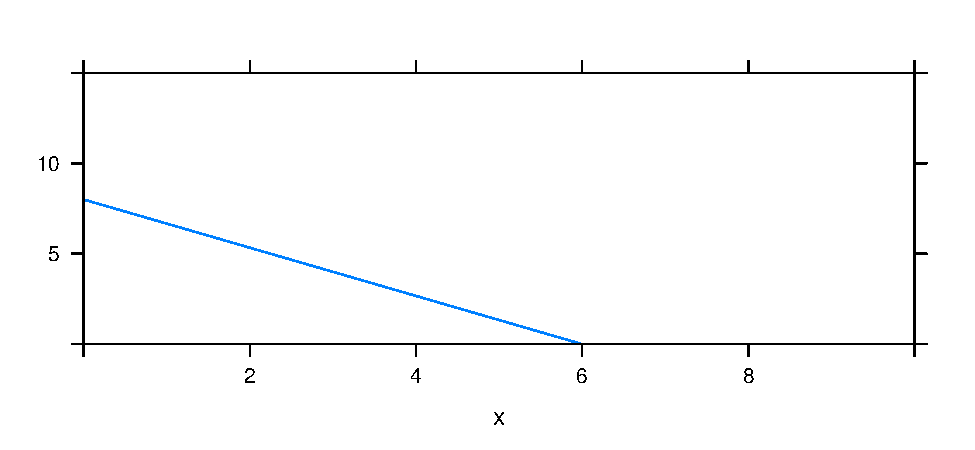
\includegraphics{Christophe_Hunt_hw6_files/figure-latex/unnamed-chunk-1-1.pdf}

We now plot the constraint \(4x - y \leq 20 ~ (hours~of~carpentry)\) as
\(y = -4x + 20\). Anything below this line is acceptable.

\begin{Shaded}
\begin{Highlighting}[]
\KeywordTok{plotFun}\NormalTok{((-}\DecValTok{4}\NormalTok{*x)+}\StringTok{ }\DecValTok{20} \NormalTok{~}\StringTok{ }\NormalTok{x, }\DataTypeTok{xlim =} \KeywordTok{c}\NormalTok{(}\DecValTok{0}\NormalTok{, }\DecValTok{10}\NormalTok{), }\DataTypeTok{ylim =} \KeywordTok{c}\NormalTok{(}\DecValTok{0}\NormalTok{,}\DecValTok{15}\NormalTok{), }
        \DataTypeTok{col =} \KeywordTok{c}\NormalTok{(}\StringTok{"red"}\NormalTok{), }\DataTypeTok{add =} \OtherTok{TRUE}\NormalTok{, }\DataTypeTok{under =} \OtherTok{TRUE}\NormalTok{,  }\DataTypeTok{ylab =} \StringTok{""}\NormalTok{)}
\end{Highlighting}
\end{Shaded}

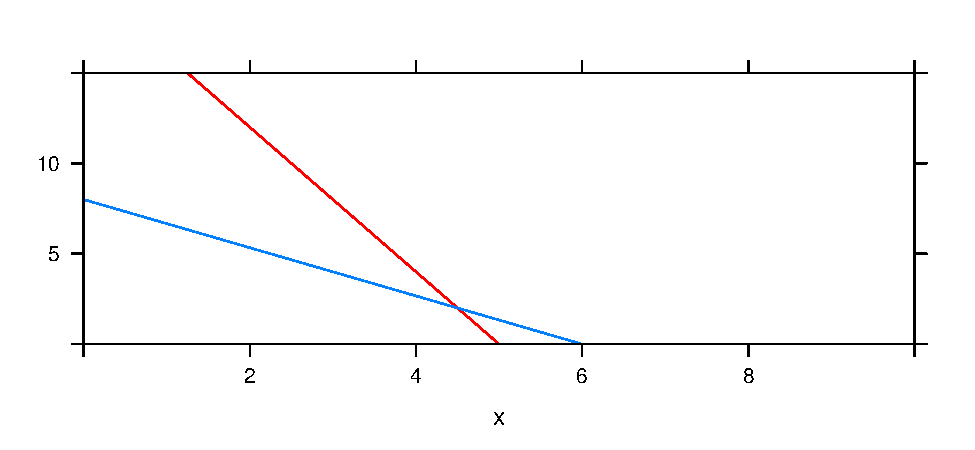
\includegraphics{Christophe_Hunt_hw6_files/figure-latex/unnamed-chunk-2-1.pdf}

We now plot the constraint \(x \geq 5 (demand)\) as \(y = 5\). Anything
above this line is acceptable.

\begin{Shaded}
\begin{Highlighting}[]
\KeywordTok{plotFun}\NormalTok{(}\DecValTok{0}\NormalTok{*x}\DecValTok{+5} \NormalTok{~}\StringTok{ }\NormalTok{x, }\DataTypeTok{xlim =} \KeywordTok{c}\NormalTok{(}\DecValTok{0}\NormalTok{, }\DecValTok{10}\NormalTok{), }\DataTypeTok{ylim =} \KeywordTok{c}\NormalTok{(}\DecValTok{0}\NormalTok{,}\DecValTok{15}\NormalTok{),}
        \DataTypeTok{col =} \KeywordTok{c}\NormalTok{(}\StringTok{"green"}\NormalTok{), }\DataTypeTok{add =} \OtherTok{TRUE}\NormalTok{, }\DataTypeTok{under =} \OtherTok{TRUE}\NormalTok{,  }\DataTypeTok{ylab =} \StringTok{""}\NormalTok{)}
\end{Highlighting}
\end{Shaded}

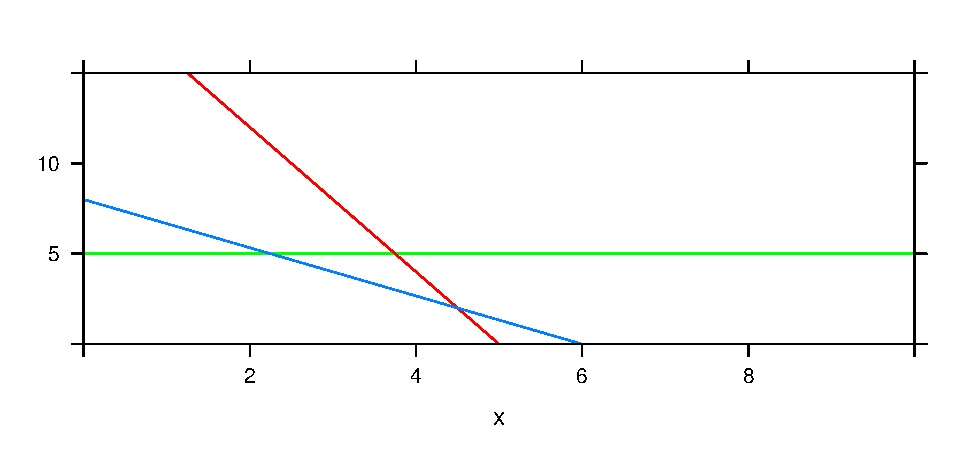
\includegraphics{Christophe_Hunt_hw6_files/figure-latex/unnamed-chunk-3-1.pdf}

As we are trying to maximize \(10x + 35y\), we look at the graph above
and the highest point within our feasibility range is (0,8). Which when
applied is 280.

\newpage

\section{Page 268: problem 6 (i.e., only question \#6 in section
7.2)}\label{page-268-problem-6-i.e.-only-question-6-in-section-7.2}

Using the \(methods\) of 7.3 solve problems 6 from section 7.2

Maximize 10x + 35y subject to

\(8x + 6y \leq 48 ~(board-feet~of~lumber)\)\\
\(4x - y \leq 20 ~ (hours~of~carpentry)\)\\
\(x \geq 5 (demand)\)\\
\(x,y \geq 0 (nonnegativity)\)

We add a ``slack'' variable

\(8x + 6y + z_1 = 48 ~(board-feet~of~lumber)\)\\
\(4x - y + z_2 = 20 ~ (hours~of~carpentry)\)\\
\(x = 5 (demand)\)\\
\(x,y, z_1, z_2 \geq 0 (nonnegativity)\)

Lets begin by setting x and y to 0 for our first intersection.

\(z_1 = 48\)\\
\(z_2 = 20\) \(0 = 5\)

\begin{quote}
This is unfeasible as x is constrained to 5.
\end{quote}

For the second intersection lets set y to 0 and z\_1 to 0.

\(8x = 48\) = \(x = 6\)\\
\(4x + z_2 = 20\) = \(24 + z _2 = 20\) = \(z_2 = -4\)

\begin{quote}
This is unfeasible as z\_2 is constrained to \(\geq\) 0 for
nonnegativity.
\end{quote}

For the third intersection lets set y to 0 and z\_2 to 0.

\(8x + z_1 = 48\) = \(40 + z_1 = 48\) = \(z_1 = 8\)\\
\(4x = 20\) = \(x = 5\)\\
\(x = 5\)

\begin{quote}
This is feasible as the intersection (0,8) does not violate any
constraints. We also know from our previous work this is the most
optimal solution.
\end{quote}

For the fourth intersection lets set x to 0 and z\_1 to 0.

\(6y = 48\) = \(y = 8\) \(-8 + z_2 = 20\) = \(z_1 = 28\) \(0 = 5\)

\begin{quote}
This is not feasible as x is constrained at 5.
\end{quote}

For the fifth intersection lets set x to 5 and z\_1 to 0.

\(40 + 6y = 48\) = \(6y = 8\) = \$y = \$ \(1\frac{1}{3}\)\\
\(20 - 1.3 + z_2 = 20\) = \$ z\_2 = \$ \(1\frac{1}{3}\)\\
\(5 = 5\)

\begin{quote}
This is not feasible as (\(1\frac{1}{3}\), \(1\frac{1}{3}\)) would not
satisfy the x = 5 condition.
\end{quote}

For the sixth intersection lets set x to 0 and z\_2 to 0.

\(6y + z_1 = 48\)\\
\(y = -20\)

\begin{quote}
This is not feasible as -20 for y violates the nonnegativity.
\end{quote}

For the seventh intersection lets set x to 5 and z\_2 to 0

\(40 + 6y + z_1 = 48\) = \(6y + z_1 = 8\) = \(z_1 = 8\)\\
\(20 - y = 20\) = \(y = 0\)

\begin{quote}
This is feasible and as previously seen is the most optimal solution. I
am interested to know if my technique is correct here. I would have
assumed that I would not get (0,8) twice using this method.
\end{quote}

\begin{quote}
I am also concerned about this method or at least my attempt to solve
this system using this method since (2.5, 5) is clearly a solution in
the graphical solution but I did not arrive at it in my algebraically
approach.
\end{quote}

\section{TODO Page 284: problem 1}\label{todo-page-284-problem-1}

For the example problems in this section, determine the sensitivity of
the optimal solution to a change in \(c_2\) using the objective function
\(25x_1 + c_2x_2\).

\begin{quote}
First we determine the slope in the \(x_1,x_2\)-plane.
\(25x_1 + c_2x_2\)\\
\(c_2x_2 = -25x_1\)\\
\(x_2 = -\frac{25}{c_2}x_1\)
\end{quote}

\begin{quote}
The slope of the first constraint is \(-\frac{2}{3}\). The slope of the
second constraint is \(-\frac{5}{4}\). Therefore, the inequality exists
as:
\end{quote}

\begin{quote}
\(-\frac{2}{3}~\leq~-\frac{25}{c_2}~\leq~-\frac{5}{4}\)
\end{quote}

\begin{quote}
We further multiply by -1 to get:
\end{quote}

\begin{quote}
\(\frac{2}{3}~\geq~\frac{25}{c_2}~\geq~\frac{5}{4}\)
\end{quote}

\begin{quote}
We can then determine the upper and lower bounds by setting our
\(\frac{25}{c_2}\) = \(\frac{2}{3}\) and \(\frac{25}{c_2}\) =
\(\frac{5}{4}\)
\end{quote}


\end{document}
